% Options for packages loaded elsewhere
\PassOptionsToPackage{unicode}{hyperref}
\PassOptionsToPackage{hyphens}{url}
\PassOptionsToPackage{dvipsnames,svgnames*,x11names*}{xcolor}
%
\documentclass[
  11pt,
]{article}
\usepackage{lmodern}
\usepackage{amssymb,amsmath}
\usepackage{ifxetex,ifluatex}
\ifnum 0\ifxetex 1\fi\ifluatex 1\fi=0 % if pdftex
  \usepackage[T1]{fontenc}
  \usepackage[utf8]{inputenc}
  \usepackage{textcomp} % provide euro and other symbols
\else % if luatex or xetex
  \usepackage{unicode-math}
  \defaultfontfeatures{Scale=MatchLowercase}
  \defaultfontfeatures[\rmfamily]{Ligatures=TeX,Scale=1}
\fi
% Use upquote if available, for straight quotes in verbatim environments
\IfFileExists{upquote.sty}{\usepackage{upquote}}{}
\IfFileExists{microtype.sty}{% use microtype if available
  \usepackage[]{microtype}
  \UseMicrotypeSet[protrusion]{basicmath} % disable protrusion for tt fonts
}{}
\makeatletter
\@ifundefined{KOMAClassName}{% if non-KOMA class
  \IfFileExists{parskip.sty}{%
    \usepackage{parskip}
  }{% else
    \setlength{\parindent}{0pt}
    \setlength{\parskip}{6pt plus 2pt minus 1pt}}
}{% if KOMA class
  \KOMAoptions{parskip=half}}
\makeatother
\usepackage{xcolor}
\IfFileExists{xurl.sty}{\usepackage{xurl}}{} % add URL line breaks if available
\IfFileExists{bookmark.sty}{\usepackage{bookmark}}{
\usepackage{hyperref}
}
\hypersetup{
  pdftitle={Table de données et fichier CSV},
  pdfauthor={Première NSI Lycée du Parc},
  colorlinks=true,
  linkcolor=Maroon,
  filecolor=Maroon,
  citecolor=Blue,
  urlcolor=Blue,
  pdfcreator={LaTeX via pandoc}}
\urlstyle{same} % disable monospaced font for URLs
\usepackage[top=20mm,left=20mm,right=20mm,heightrounded]{geometry}
\usepackage{listings}
\newcommand{\passthrough}[1]{#1}
\lstset{defaultdialect=[5.3]Lua}
\lstset{defaultdialect=[x86masm]Assembler}
\usepackage{graphicx}
\makeatletter
\def\maxwidth{\ifdim\Gin@nat@width>\linewidth\linewidth\else\Gin@nat@width\fi}
\def\maxheight{\ifdim\Gin@nat@height>\textheight\textheight\else\Gin@nat@height\fi}
\makeatother
% Scale images if necessary, so that they will not overflow the page
% margins by default, and it is still possible to overwrite the defaults
% using explicit options in \includegraphics[width, height, ...]{}
\setkeys{Gin}{width=\maxwidth,height=\maxheight,keepaspectratio}
% Set default figure placement to htbp
\makeatletter
\def\fps@figure{htbp}
\makeatother
\setlength{\emergencystretch}{3em} % prevent overfull lines
\providecommand{\tightlist}{%
  \setlength{\itemsep}{0pt}\setlength{\parskip}{0pt}}
\setcounter{secnumdepth}{5}

\title{Table de données et fichier CSV}
\usepackage{etoolbox}
\makeatletter
\providecommand{\subtitle}[1]{% add subtitle to \maketitle
  \apptocmd{\@title}{\par {\large #1 \par}}{}{}
}
\makeatother
\subtitle{Traitement de données en tables}
\author{Première NSI Lycée du Parc}
\date{}

%%%jolis boites

\usepackage{fancybox, graphicx}



%%%%%%%%%%%%%%%%Packages et Macros Frederic%%%%%%%%%%%%%%%%%%%%%%%%%%%%%


%%%%Insertion de liens hypertextes %%%%

            
%%%%%%%%%%PSTricks%%%%%%%%%%%%

\usepackage{pstricks,pst-plot,pst-text,pst-tree,pst-eps,pst-fill,pst-node,pst-math,pstricks-add,pst-xkey,pst-eucl}


%%%%%%%Tikz%%%%%%%%%%%%%%%
\usepackage{pgf,tikz,tkz-tab}
% Pour les tableaux de signes ou de variations avec tkz-tab voir https://zestedesavoir.com/tutoriels/439/des-tableaux-de-variations-et-de-signes-avec-latex/#1-13389_tikz-un-package-qui-en-a-dans-le-ventre
\usetikzlibrary{arrows}
\usetikzlibrary{shapes.geometric}
\usetikzlibrary{shapes.geometric}
\usetikzlibrary{petri}
\usetikzlibrary{decorations}
\usetikzlibrary{arrows}
\usetikzlibrary{math}
 %Variables must be declared in a tikzmath environment but
       % can be used outside
%       \tikzmath{int \n; \n = 508; \x1 = 1; \y1 =1; 
%                   %computations are also possible
%                    \x2 = \x1 + 1; \y2 =\y1 +3; } 


%%%%%%%%%%%%%%%%%%%%%%%%%%%%%%%%%%%%%%%%
%%%%%%%%%%%Commandes Tikz Perso%%%%%%%%%%%%%%%

% Définition des nouvelles options xmin, xmax, ymin, ymax
% Valeurs par défaut : -3, 3, -3, 3
\tikzset{
xmin/.store in=\xmin, xmin/.default=-3, xmin=-3,
xmax/.store in=\xmax, xmax/.default=3, xmax=3,
ymin/.store in=\ymin, ymin/.default=-3, ymin=-3,
ymax/.store in=\ymax, ymax/.default=3, ymax=3,
}
% Commande qui trace la grille entre (xmin,ymin) et (xmax,ymax)
\newcommand {\grille}[2]
{\draw[help lines,black, thick] (\xmin,\ymin) grid[xstep=#1, ystep=#2] (\xmax,\ymax);}
% Commande \axes
\newcommand {\axes} {
\draw[->,very thick] (\xmin,0) -- (\xmax,0);
\draw[->,very thick] (0,\ymin) -- (0,\ymax);
\draw (0.95*\xmax, 0) node[above] {};
\draw (0, 0.95*\ymax) node[left] {};
}
% Commande qui limite l?affichage à (xmin,ymin) et (xmax,ymax)
\newcommand {\fenetre}
{\clip (\xmin,\ymin) rectangle (\xmax,\ymax);}

%Exemple d'utilisation

%\begin{center}
%\begin{tikzpicture} [xmin=-2,xmax=2,ymin=0,ymax=5]
%\grille{1} \axes \fenetre
%\draw plot[smooth] (\x,\x^2);
%\end{tikzpicture}
%\end{center}

%style pour la perspective cavalière française
%voir Tikz pour l'impatient page 68
\tikzset{math3d/.style=
{x= {(-0.353cm,-0.353cm)}, z={(0cm,1cm)},y={(1cm,0cm)}}}

%%%%%%%Symbole pour code calculatrice%%%%%%

%Flèche remplie pour défilement de menu

\newcommand{\flechefillright}{

\begin{tikzpicture}[scale=0.15] \fill (0,0)--(2,1)--(0,2)--cycle;
\end{tikzpicture}}

%%%%%%%%%%%%%Symboles pour calculatrice Casio%%%%
\newcommand{\execasio}{\Pisymbol{psy}{191}} %Retour chariot
\newcommand{\dispcasio}{\begin{pspicture}(.1,.1)\pspolygon*(.1,0)(.1,.1)\end{pspicture}} %Triangle « Disp »
\newcommand{\dispcasiotikz}{
\begin{tikzpicture}[scale=0.2]
\fill (0,0) -- (1,0) -- (1,1) -- cycle;
\end{tikzpicture}} %Triangle « Disp »
%

%Fleche entre deux lignes, d'apres 'un bon petit' : http://forum.mathematex.net/latex-f6/fleches-entre-deux-lignes-pour-resolution-d-equation-t10283.html#p99817
\newcommand\addnode[1]{\Rnode{#1}{}}
\newcommand\linknode[3]{\ncbar[angleA=0,angleB=0,nodesep=1ex,arm=10ex,offset=-2pt]{->}{#1}{#2}\Aput{\vphantom{x}#3}}


%%Commande pour touche de calculatrice

\newcommand\tc[1]{%
{
\begin{tikzpicture}
\node[draw,rectangle,rounded corners=3pt] (P) at (0,0){#1};
\end{tikzpicture}
}
}

%%%%%%%%%%%%%%%%%%%%%%%%%%%%%%%%%%%%%%%%
%%%%%%%%%%%Fin Commandes Tikz%%%%%%%%%%%%%%%


%%%%%%%%%%%%Specifiques%%%%%%%%%%%
\usepackage{wrapfig}
%pour insérer une figure à droite ou à gauche d'un texte
%\begin{wrapfigure}[nb lignes]{placement l,r,c,i(inside),o(outside)}[overhang]{width}
%ce package fonctionne mal à proximité des listes
%%%%%%%%%%%%%%%%%%%%%%%%%%%%%%%%%%%%%

%%%%%Environnements et symboles spéciaux pour faire joli%%%%%%

%%%Bclogo, pour des environnements + jolis avec insertion de logo%%%%
%Dépendances de  bclogo
\usepackage{xkeyval}  
\usepackage{etoolbox}
\usepackage{ifpdf}
\usepackage[framemethod=tikz]{mdframed}
\usepackage[tikz]{bclogo}

%\newcommand\bcpython{\includegraphics[width=17pt]{/home/fjunier/Maths/python-logo.eps}}
\newcommand\bcpython{\includegraphics[width=17pt]{/home/fjunier/Maths/python-logo.png}}
%\newcommand\bcpython{\includegraphics[width=17pt]{/home/frederic/Maths/python-logo.png}}

%% Framed
\usepackage{framed}  %Le package « framed» Crée 3 nouveaux environnements, qui se comportent comme des minipage de largeur \linewidth, mais permettant en plus de se casser entre plusieurs pages.     * framed : avec un cadre autour;     * shaded : avec un fonc coloré (il faut définir la couleur shadecolor);     * leftbar : avec une barre le long du côté gauche.

%%%%%%%%%%%%%%%%%%%Présentation de codes sources%%%%%%%%%%%%%%%%%
\usepackage{listings}
%On utilise l?environnement lstlisting pour insérer
%un code source.
%En plus de l?environnement lstlisting, on peut également utiliser la
%commande \lstinline qui fonctionne comme la commande \verb, en ce
%sens qu?on peut utiliser n?importe quel caractère comme délimiteur. Enfin,
%la commande \lstinputlisting permet de charger un code source depuis
%un fichier externe.
%Il y a deux manières de préciser des options : soit via l?option de l?envi-
%ronnement ou de la commande, soit en utilisant la commande \lstset
%qui permet de définir des options de manière globale.

\lstset{ %
  language=Python,                % the language of the code
  basicstyle=\ttfamily,           % the size of the fonts that are used for the code
  %numbers=left,                   % where to put the line-numbers
  numberstyle=\tiny,  % the style that is used for the line-numbers
  %stepnumber=2,                   % the step between two line-numbers. If it's 1, each line 
                                  % will be numbered
  %numbersep=5pt,                  % how far the line-numbers are from the code
  backgroundcolor=\color{white},      % choose the background color. You must add \usepackage{color}
  showspaces=false,               % show spaces adding particular underscores
  showstringspaces=false,         % underline spaces within strings
  showtabs=false,                 % show tabs within strings adding particular underscores
  frame=single,                   % adds a frame around the code
  rulecolor=\color{black},        % if not set, the frame-color may be changed on line-breaks within not-black text (e.g. comments (green here))
  tabsize=4,                      % sets default tabsize to 2 spaces
  captionpos=b,                   % sets the caption-position to bottom
  breaklines=true,                % sets automatic line breaking
  breakatwhitespace=false,        % sets if automatic breaks should only happen at whitespace
  %title=\lstname,                   % show the filename of files included with \lstinputlisting;
                                  % also try caption instead of title
  breakindent=1cm,
  keywordstyle=\color{blue},          % keyword style
  commentstyle=\color{red},       % comment style
  %stringstyle=\ttfamily\color{green},         % string literal style
  escapeinside={\%*}{*)},            % if you want to add LaTeX within your code
  morekeywords={*,...},              % if you want to add more keywords to the set
  deletekeywords={...}              % if you want to delete keywords from the given language
  upquote=true,columns=flexible,
xleftmargin=1cm,xrightmargin=1cm,
 inputencoding=utf8,			%Les lignes qui suivent sont pour le codage utf8
  extendedchars=true,
  literate=%
            {é}{{\'{e}}}1
            {è}{{\`{e}}}1
            {ê}{{\^{e}}}1
            {ë}{{\¨{e}}}1
            {û}{{\^{u}}}1
            {ù}{{\`{u}}}1
            {â}{{\^{a}}}1
            {à}{{\`{a} }}1
            {î}{{\^{i}}}1
            {ô}{{\^{o}}}1
            {ç}{{\c{c}}}1
            {Ç}{{\c{C}}}1
            {É}{{\'{E}}}1
            {Ê}{{\^{E}}}1
            {À}{{\`{A}}}1
            {Â}{{\^{A}}}1
            {Î}{{\^{I}}}1
}

\lstdefinestyle{rond}{
  numbers=none,
  backgroundcolor=\color{gristclair},
  frameround =tttt
}

\lstdefinestyle{compil}{
  numbers=none,
  backgroundcolor=\color{gristclair}
}
%\lstset{language=Python,basicstyle=\small , frame=single,tabsize=4,showspaces=false,showtabs=false,showstringspaces=false,numbers=left,numberstyle=\tiny , extendedchars=true}



%%%%%%%%%%%%%%%%%%%%%%%%%%%%%%%%%%%%%%%%%%%%%%%%%%%%%%%%%%%%%%%%%%%%%%%%
%%%%%%%%%%%%%%%%%%%%Environnements persos%%%%%%%%%%%%%%%%%%%%%%%%%%%%%%%%
%Syntaxe :
%\newenvironment{nom}[nombre d'args][defaut]{definitions initiales}{definitions finales}
%definitions intiales sont les commandes appelées par \begin{nom}
%Definitions finales sont les commandes appelées par \end{nom}

%%%%%%%%%%%%%%%%Définitions des environnemts persostheoreme, exemple ..%%%%
%%%% Exercice avec encadré %%%%
\newcounter{exo}
\newenvironment{exercice}[1]
{\par \medskip   \addtocounter{exo}{1} \noindent  
\begin{bclogo}[arrondi =0.1,   noborder = true, logo=\bccrayon, marge=4]{~\textbf{Exercice} \textbf{\theexo} {\itshape #1} }  \par}
{
\end{bclogo}
 \par \bigskip }

%%Axiomes, Theoremes, Propriété, Définition, Methode, Preuve


\newenvironment{axiome}[1]
{\par \medskip   \begin{leftbar} \noindent \underline{\textbf{Axiome}}\hspace{0.5cm}{\itshape #1}   \vspace*{10pt} \par }
{\end{leftbar}  \par \medskip }


\newcounter{thme}
\newenvironment{theoreme}[1]
{\par \medskip  \addtocounter{thme}{1} \noindent  
\begin{bclogo}[arrondi =0.1,  ombre = true, barre=none, logo=\bcbook, marge=4]{~\textbf{Théorème} \textbf{\thethme} {\itshape #1} }   \par}
{
\end{bclogo}
 \par \bigskip}

 \newenvironment{theoremedef}[1]
{\par \medskip   \addtocounter{thme}{1} \noindent  
\begin{bclogo}[arrondi =0.1,  ombre = true, barre=none, logo=\bcbook, marge=4]{~\textbf{Théorème-Définition} \textbf{\thethme} {\itshape #1} }   \par}
{
\end{bclogo}
 \par \bigskip }
 
\newcounter{prop}
\newenvironment{propriete}[1]
{\par \medskip   \addtocounter{prop}{1} \noindent  
\begin{bclogo}[arrondi =0.1,  ombre = true, barre=none, logo=\bcbook, marge=4]{~\textbf{Propriété} \textbf{\theprop} {\itshape #1} }   \par}
{
\end{bclogo}
 \par \bigskip }


\newenvironment{corollaire}[1]
{\par \medskip   \noindent  
\begin{bclogo}[arrondi =0.1,  ombre = true, barre=none, logo=\bcbook, marge=4]{~\textbf{Corollaire} {\itshape #1} } \par }
{
\end{bclogo}
 \par \bigskip }

\newenvironment{demo}[1]
{\par \medskip   \noindent  
\begin{bclogo}[arrondi =0.1,  ombre = true, barre=zigzag, noborder = true, logo=\bcloupe, marge=0]{~\textbf{Démonstration} {\itshape #1} } \par \vspace{10pt}}
{
\end{bclogo}
 \par \bigskip }

\newcounter{activite}
\newenvironment{activite}[1]
{\par \medskip   \noindent   \addtocounter{activite}{1}
\begin{bclogo}[arrondi =0.1,   noborder = true, logo=\bcvelo, marge=4]{~\textbf{Activité} \textbf{\theactivite} {\itshape #1} }  \par}
{
\end{bclogo}
 \par \bigskip }


\newenvironment{synthese}
{\par \medskip   \noindent   
\begin{bclogo}[arrondi =0.1,   noborder = true, logo=\bccle, marge=4]{~\textbf{Synthèse}   }  \par}
{
\end{bclogo}
 \par \bigskip }
 
 
\newcounter{rque}
\newenvironment{remarque}
{\par \medskip    \addtocounter{rque}{1} \noindent  
\begin{bclogo}[arrondi =0.1,  ombre = true, barre=snake, noborder = true, logo=\bcinfo, marge=0]{~\textbf{Remarque} \textbf{\therque}}  \par }
{
\end{bclogo}
 \par \bigskip }

\newcounter{def}
\newenvironment{definition}[1]
{\par \medskip   \addtocounter{def}{1} \noindent  
\begin{bclogo}[arrondi =0.1,  ombre = true, barre=none, logo=\bcbook, marge=4]{~\textbf{Définition} \textbf{\thedef} {\itshape #1} }  \par}
{
\end{bclogo}
 \par \bigskip }
 
 
 \newcounter{cours}
\newenvironment{cours}[1]
{\par \medskip   \addtocounter{cours}{1} \noindent  
\begin{bclogo}[arrondi =0.1,  ombre = true, barre=none, logo=\bcbook, marge=4]{~\textbf{Point de cours} \textbf{\thecours} {\itshape #1} }  \par}
{
\end{bclogo}
 \par \bigskip }
 
 

\newenvironment{introduction}
{\par \medskip    \noindent  
 \begin {bclogo}[couleur = blue!5 , arrondi =0.1,logo=\bcrosevents, marge=4] {~\textbf{Introduction}    }
 \par }
{
\end{bclogo}
 \par \bigskip }
 
\newenvironment{memo}[1]
{\par \medskip    \noindent  
\begin{bclogo}[arrondi =0.1,  ombre = true, barre=none, logo=\bccle, marge=4]{~\textbf{À retenir}  {\itshape #1} }  \par}
{
\end{bclogo}
 \par \bigskip }
 
\newcounter{exple}
\newenvironment{exemple}[1]
{\par \medskip   \addtocounter{exple}{1} \noindent  
\begin{bclogo}[arrondi =0.1,   noborder = true, logo=\bclampe, marge=4]{~\textbf{Exemple} \textbf{\theexple} {\itshape #1} }  \par}
{
\end{bclogo}
 \par \bigskip }




\newcounter{alg}
\newenvironment{algorithme}[1]
{\par \medskip   \addtocounter{alg}{1} \noindent  
 \begin {bclogo}[noborder = true, barre=zigzag,logo=\bcpython, marge=4] {~\textbf{Algorithmique} \textbf{\thealg} {\itshape #1} }  \par}
{
\end{bclogo}
 \par \bigskip }

\newcounter{prog}
\newenvironment{programme}[1]
{\par \medskip   \addtocounter{prog}{1} \noindent  
 \begin {bclogo}[noborder = true, barre=zigzag,logo=\bcpython, marge=4] {~\textbf{Programme} \textbf{\theprog} {\itshape #1} }  \par  \bigskip}
{
\end{bclogo}
 \par \bigskip }
 
\newcounter{logi}
\newenvironment{logique}[1]
{\par \medskip   \addtocounter{logi}{1} \noindent  
 \begin {bclogo}[noborder = true, barre=zigzag,logo=\bclampe, marge=4] {~\textbf{Logique} \textbf{\thelogi} {\itshape #1} }  \par}
{
\end{bclogo}
 \par \bigskip }


\newenvironment{methode}[1]
{\par \medskip    \noindent  
 \begin {bclogo}[arrondi =0.1,logo=\bcoutil, marge=4,noborder = true] {~\textbf{Méthode}   {\itshape #1} }  \par}
{
\end{bclogo}
 \par \bigskip }


\newcounter{histo}
\newenvironment{histoire}[1]
{\par \medskip   \addtocounter{histo}{1} \noindent  
 \begin {bclogo}[couleur = blue!10 , arrondi =0.1,logo=\bchorloge, marge=4] {~\textbf{Histoire} \textbf{\thehisto} {\itshape #1} }  \par}
{
\end{bclogo}
 \par \bigskip }




%Environnement contenu pour un document présentant une progression annuelle
\newenvironment{contenu}
{\par \medskip   \begin {bclogo}[ noborder = true,logo=\bccrayon] \noindent {\large \textbf{Contenu de la séance}} \vspace*{10pt} \par  }
{\end{bclogo}  \par \medskip }

%Environnement programme pour un document présentant une progression annuelle
%\newenvironment{programme}
%{\par \medskip   \begin {bclogo}[ noborder = true, barre=zigzag,logo=\bcinfo] \noindent {\large \textbf{Programme officiel}} \vspace*{10pt} \par  }
%{\end{bclogo}  \par \medskip }

%Environnement programme pour un document présentant une progression annuelle
\newenvironment{ressource}
{\par \medskip   \begin {bclogo}[ noborder = true,logo=\bcbook] \noindent {\large \textbf{Ressources}}\\vspace*{10pt} \par }
{\end{bclogo}  \par \medskip }




%%%%%%%%%%%%%%%%%%Maths divers%%%%%%%%%%%%%%%%%%%%%%%%%
%%%%%%%%%%%%%Nombres%%%%%%%%%%%%%%%%

%Ensemble prive de...
%\newcommand{\prive}{\boi}%{\backslash}

%Ensembles de nombres%%%%%%%%%%%%%%%%%
\newcommand{\R}{\mathbb{R}}
\newcommand{\N}{\mathbb{N}}
\newcommand{\D}{\mathbb{D}}
\newcommand{\Z}{\mathbb{Z}}
\newcommand{\Q}{\mathbb{Q}}
%\newcommand{\C}{\mathbb{C}}
\newcommand{\df}{~\ensuremath{]0;+\infty[}~}
\newcommand{\K}{\mathbb{K}}

%%%%%%%%Arithmetique%%%%%%%%%%
%PGCD, PPCM
\newcommand{\PGCD}{\mathop{\rm PGCD}\nolimits}
\newcommand{\PPCM}{\mathop{\rm PPCM}\nolimits}

%Intervalles
\newcommand{\interoo}[2]{]#1\, ;\, #2[}
\newcommand{\Interoo}[2]{\left]#1\, ;\, #2\right[}
\newcommand{\interof}[2]{]#1\, ;\, #2]}
\newcommand{\Interof}[2]{\left]#1\, ;\, #2\right]}
\newcommand{\interfo}[2]{[#1\, ;\, #2[}
\newcommand{\Interfo}[2]{\left[#1\, ;\, #2\right[}
\newcommand{\interff}[2]{[#1\, ;\, #2]}
\newcommand{\Interff}[2]{\left[#1\, ;\, #2\right]}
%\newcommand\interentiers #1#2{[\! [#1\, ;\, #2]\! ]}
\newcommand{\interentiers}[2]{\llbracket #1\, ;\, #2\rrbracket}
%


%%%%%%%%%%%%%%Nombres complexes%%%%%

\newcommand{\ic}{\text{i}}
%\newcommand{\I}{\text{i}}
\newcommand{\im}[1]{\text{Im}\left(#1\right)}
\newcommand{\re}[1]{\text{Re}\left(#1\right)}
\newcommand{\Arg}[1]{\text{arg}\left(#1\right)}
\newcommand{\Mod}[1]{\left[#1\right]}
%Parties entière, réelle, imaginaire, nombre i
\newcommand{\ent}[1]{\text{E}\left(#1\right)}
\renewcommand{\Re}{\mathop{\rm Re}\nolimits}
\renewcommand{\Im}{\mathop{\rm Im}\nolimits}
\renewcommand{\i}{\textrm{i}}

%%%%%%%%%%%Probabilites et statistiques%%%%%
\newcommand{\loibinom}[2]{\mathcal{B}\left(#1\ ; \ #2 \right)}
\newcommand{\loinorm}[2]{\mathcal{N}\left(#1\ ; \ #2 \right)}
\newcommand{\loiexp}[1]{\mathcal{E}\left(#1\right)}
\newcommand{\proba}[1]{\mathbb{P}\big(#1\big)}
\newcommand{\probacond}[2]{\mathbb{P}_{#2}\big(#1\big)}
\newcommand{\esperance}[1]{\mathbb{E}\left(#1\right)}
\newcommand{\variance}[1]{\mathbb{V}\left(#1\right)}
\newcommand{\ecart}[1]{\sigma\left(#1\right)}
\newcommand{\dnormx}{\frac{1}{\sqrt{2\pi}} \text{e}^{-\frac{x^2}{2}}}
\newcommand{\dnormt}{\frac{1}{\sqrt{2\pi}} \text{e}^{-\frac{t^2}{2}}}

%Covariance
\newcommand{\cov}{\mathop{\rm cov}\nolimits}
%


%%%%%%%%%%Analyse%%%%%%%%%%%

%%%%%%%%%%%Courbe%%%%%%%%%%%%
\newcommand{\courbe}[1]{\ensuremath{\mathcal{C}_{#1}}}

%%%%%%%Fonction exponentielle%%%%%
\newcommand{\fe}{~fonction exponentielle~}
\newcommand{\e}{\text{e}}

%Fonction cotangente
\newcommand{\cotan}{\mathop{\rm cotan}\nolimits}
%%%%%%%%%%%%%%%%%%%%%%%%%%%%%%%%%%%%%%%%%
%
%Fonctions hyperboliques
\newcommand{\ch}{\mathop{\rm ch}\nolimits}
\newcommand{\sh}{\mathop{\rm sh}\nolimits}


%%%%%%%%%%%%%%Limites%%%%%%
\newcommand{\limite}[2]{\lim\limits
_{x \to #1} #2}
\newcommand{\limitesuite}[1]{\lim\limits
_{n \to +\infty} #1}
\newcommand{\limiteg}[2]{\lim\limits
_{\substack{x \to #1 \\ x < #1 }} #2}
\newcommand{\limited}[2]{\lim\limits
_{\substack{x \to #1 \\ x > #1 }} #2}

%%%%%%%%%%Continuité%%%%%%%%%%%
\newcommand{\TVI}{théorème des valeurs intermédiaires}

%%%%%%%%%%%Suites%%%%%%%%%%%%
\newcommand{\suite}[1]{\ensuremath{\left(#1_{n}\right)}}
\newcommand{\Suite}[2]{\ensuremath{\left(#1\right)_{#2}}}
%

%%%%%%%%%%%%%%%Calcul intégral%%%%%%
\newcommand{\dx}{\ensuremath{\text{d}x}}		% dx
\newcommand{\dt}{\ensuremath{\text{d}t}}		% dt
\newcommand{\dtheta}{\ensuremath{\text{d}\theta}}		% dtheta
\newcommand{\dy}{\ensuremath{\text{d}y}}		% dy
\newcommand{\dq}{\ensuremath{\text{d}q}}		% dq

%%%Intégrale%%%
\newcommand{\integralex}[3]{\int_{#1}^{#2} #3 \ \dx}
\newcommand{\integralet}[3]{\int_{#1}^{#2} #3 \ \dt}
\newcommand{\integraletheta}[3]{\int_{#1}^{#2} #3 \ \dtheta}

%%%%%Equivalent%%
\newcommand{\equivalent}[1]{\build\sim_{#1}^{}}

%o et O%%%%
\renewcommand{\o}[2]{\build o_{#1\to #2}^{}}
\renewcommand{\O}[2]{\build O_{#1\to #2}^{}}



%%%%%%%%%%%%%%%Geometrie%%%%%%%%%%%%%%%%%%%%%%%

%%%%%%%%%%%%%%%Reperes%%%%%%%%%%%%%%
\def\Oij{\ensuremath{\left(\text{O},~\vect{\imath},~\vect{\jmath}\right)}}
\def\Oijk{\ensuremath{\left(\text{O},~\vect{\imath},~ \vect{\jmath},~ \vect{k}\right)}}
\def\Ouv{\ensuremath{\left(\text{O},~\vect{u},~\vect{v}\right)}}
\renewcommand{\ij}{(\vec\imath\, ;\vec\jmath\,)}
\newcommand{\ijk}{(\vec\imath\, ;\vec\jmath\, ;\vec k\,)}
\newcommand{\OIJ}{(O\,;\, I\,;\, J\,)}
\newcommand{\repere}[3]{\big(#1\, ;\,\vect{#2} ;\vect{#3}\big)}
\newcommand{\reperesp}[4]{\big(#1\, ;\,\vect{#2} ;\vect{#3} ;\vect{#4}\big)}

%%%%%%%%%Coordonnees%%%%%%%%%%%%%%
\newcommand{\coord}[2]{(#1\, ;\, #2)}
\newcommand{\bigcoord}[2]{\big(#1\, ;\, #2\big)}
\newcommand{\Coord}[2]{\left(#1\, ;\, #2\right)}
\newcommand{\coordesp}[3]{(#1\, ;\, #2\, ;\, #3)}
\newcommand{\bigcoordesp}[3]{\big(#1\, ;\, #2\, ;\, #3\big)}
\newcommand{\Coordesp}[3]{\left(#1\, ;\, #2\, ;\, #3\right)}
\newcommand{\Vcoord}[3]{\begin{pmatrix} #1 \\ #2 \\ #3 \end{pmatrix}}
%Symboles entre droites
%\newcommand{\paral}{\sslash}
\newcommand{\paral}{\mathop{/\!\! /}}
%

%%%%%%%%%Produit scalaire, Angles%%%%%%%%%%
\newcommand{\scal}[2]{\vect{#1} \, \cdot \, \vect{#2}}
\newcommand{\Angle}[2]{\left(\vect{#1} \, , \, \vect{#2}\right)}
\newcommand{\Anglegeo}[2]{\left(\widehat{\vect{#1} \, ; \, \vect{#2}}\right)}
\renewcommand{\angle}[1]{\widehat{#1}}
\newcommand{\anglevec}[2]{\left(\vect {#1}\, ,\,\vect {#2} \right)}
\newcommand{\anglevecteur}[2]{(#1\, , \, #2)}
\newcommand{\Anglevec}[2]{(\vecteur{#1}\, ,\,\vecteur{#2})}
\newcommand{\prodscal}[2]{#1 \, \cdot \, #2}
%


%Arc
%\newcommand{\arc}[1]{\wideparen{#1}}
\newcommand{\arcoriente}[1]{\overset{\curvearrowright}{#1}}
%
%


%%%%%%%%%%%%%%%Normes%%%%%%%%%%%%%%%%
\newcommand{\norme}[1]{\left\| #1\right\|}
\newcommand{\normebis}[1]{\delim{2pt}{\|}{9pt}\! #1\delim{2pt}{\|}{9pt}}
\newcommand{\normetriple}[1]{\left |\kern -.07em\left\| #1\right |\kern -.07em\right\|}
\newcommand{\valabs}[1]{\big| \, #1 \, \big|}
%

%%%%%%%%%%%%%%%%%%%%%%%%%%%Degré%%%%%%
%\newcommand{\Degre}{\ensuremath{^\circ}}
%La commande \degre est déjà définie dans le package babel

%%%%%%%%%%Vecteurs%%%%%%%%%%%
\newcommand{\vect}[1]{\mathchoice%
{\overrightarrow{\displaystyle\mathstrut#1\,\,}}%
{\overrightarrow{\textstyle\mathstrut#1\,\,}}%
{\overrightarrow{\scriptstyle\mathstrut#1\,\,}}%
{\overrightarrow{\scriptscriptstyle\mathstrut#1\,\,}}}



%%%%%%%%%%%%%Algebre%%%%%%%%%%%%%%%


%%%%%%%%%%Systemes%%%%%%%%%%%
%Systemes
\newcommand{\sys}[2]{
\left\lbrace
 \begin{array}{l}
  \negthickspace\negthickspace #1\\
  \negthickspace\negthickspace #2\\
 \end{array}
\right.\negthickspace\negthickspace}
\newcommand{\Sys}[3]{
\left\lbrace
 \begin{array}{l}
  #1\\
  #2\\
  #3\\
 \end{array}
\right.}
\newcommand{\Sysq}[4]{
\left\lbrace
 \begin{array}{l}
  #1\\
  #2\\
  #3\\
  #4\\
 \end{array}
\right.}
%
%

%%%%%%%%%%%%%%%%Matrices%%%%%%%%%%%%%%%%%%
%Comatrice
\newcommand{\com}{\mathop{\rm com}\nolimits}
%
%
%Trace
\newcommand{\tr}{\mathop{\rm tr}\nolimits}
%
%
%Transposee
\newcommand{\transposee}[1]{{\vphantom{#1}}^t\negmedspace #1}
%
%
%Noyau
\newcommand{\Ker}{\mathop{\rm Ker}\nolimits}
%
%

%
%Matrices
\newcommand{\Mn}{\mathcal M_n}
\newcommand{\matrice}[4]{
\left(
 \begin{array}{cc}
  #1 & #2 \\
  #3 & #4
 \end{array}
\right)}

\newcommand{\Matrice}[9]{
\left(
 \begin{array}{ccc}
  #1 & #2 & #3\\
  #4 & #5 & #6\\
  #7 & #8 & #9
 \end{array}
\right)}
\newcommand{\Vect}[3]{
\left(\negmedspace
 \begin{array}{c}
  #1\\
  #2\\
  #3
 \end{array}\negmedspace
\right)}
\newcommand{\Ideux}{\matrice{1}{0}{0}{1}}
\newcommand{\Itrois}{\Matrice{1}{0}{0}{0}{1}{0}{0}{0}{1}}
%
%
%Determinants
\newcommand{\determinant}[4]{
\left|
 \begin{array}{cc}
  #1 & #2 \\
  #3 & #4
 \end{array}
\right|}
\newcommand{\Determinant}[9]{
\left|
 \begin{array}{ccc}
  #1 & #2 & #3\\
  #4 & #5 & #6\\
  #7 & #8 & #9
 \end{array}
\right|}

\begin{document}
\maketitle

\renewcommand*\contentsname{Table des matières}
{
\hypersetup{linkcolor=}
\setcounter{tocdepth}{3}
\tableofcontents
}
\hypertarget{cruxe9dits}{%
\section*{Crédits}\label{cruxe9dits}}
\addcontentsline{toc}{section}{Crédits}

\emph{Ce cours est largement inspiré de deux sources :}

\begin{itemize}
\tightlist
\item
  \emph{le chapitre 15 du manuel NSI de la collection Tortue chez
  Ellipse, auteurs : Ballabonski, Conchon, Filliatre, N'Guyen ;}
\item
  \emph{le cours de Julien de Villèle}.
\end{itemize}

\hypertarget{table-de-donnuxe9es}{%
\section{Table de données}\label{table-de-donnuxe9es}}

\begin{histoire}{}

L'homme organisait les données sous forme de tableau bien avant
l'invention de l'ordinateur : les \textbf{données tabulaires} ou
\textbf{tables de données}, apparaissent déjà dans les livres de compte
de l'Égypte ancienne. De nos jours les relevés de comptes bancaires sont
encore présentés sous forme de tableaux avec pour chaque opération sa
date, sa nature (débit ou crédit) et son montant.

En informatique, les \textbf{tables de données} se sont développées dans
dans les années 1970 avec l'essor des
\href{https://fr.wikipedia.org/wiki/Syst\%C3\%A8me_de_gestion_de_base_de_donn\%C3\%A9es}{Systèmes
de Gestion de Base de Données} s'appuyant sur le \textbf{modèle
relationnel} proposé par
\href{https://fr.wikipedia.org/wiki/Edgar_Frank_Codd}{Edgar F. Codd}
chez IBM. Les
\href{https://fr.wikipedia.org/wiki/Syst\%C3\%A8me_de_gestion_de_base_de_donn\%C3\%A9es}{Systèmes
de Gestion de Base de Données} permettent aujourd'hui le traitement
automatique de gigantesques bases de données, qui est un élément
fondamental dans nos sociétés de l'information.

Les
\href{https://fr.wikipedia.org/wiki/Syst\%C3\%A8me_de_gestion_de_base_de_donn\%C3\%A9es}{Systèmes
de Gestion de Base de Données} seront étudiés en classe de terminale.
Nous présenterons cette année les traitements de \textbf{tables de
données} qui peuvent être effectués à l'aide de scripts Python, ce qui
couvre déjà un large champ de besoins en \emph{data science},
\emph{bio-informatique}, \emph{informatique financière ou de gestion}
\ldots{}

\end{histoire}

\begin{definition}{}

Une feuille de tableur est un modèle de \textbf{données tabulaires} ou
\textbf{table de données}.

Définissons le vocabulaire :

\begin{itemize}
\item
  Une \textbf{table}, représentée sous forme de tableau, est une
  collection d'éléments qui sont les lignes du tableau.
\item
  Chaque élément de la \textbf{table}, ou ligne de sa représentation
  sous forme de tableau, s'appelle un \textbf{enregistrement}.
\item
  Tous les \textbf{enregistrements} d'une même \textbf{table} sont des
  \textbf{p-uplets nommés} qui partagent les mêmes
  \textbf{descripteurs}, appelés aussi \textbf{attributs}. Dans une
  représentation de la \textbf{table} sous forme de tableau, chaque
  \textbf{attribut} correspond à une colonne. Chaque \textbf{attribut}
  est caractérisé par son \textbf{type} et son \textbf{domaine de
  valeurs}.
\item
  Dans une représentation sous forme de tableau, les
  \textbf{descripteurs} ou \textbf{attributs} sont en général placés
  comme en-tête de colonnes sur la première ligne.
\end{itemize}

\end{definition}

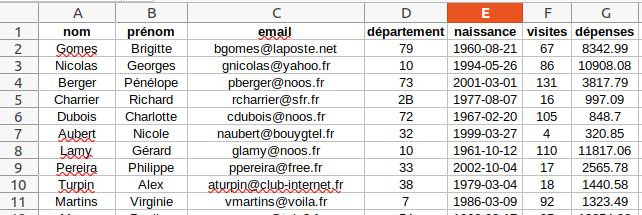
\includegraphics{images/tableur.png}\\

\begin{exemple}{}

La table représentée ci-dessus rassemble les enregistrements des clients
d'un site web marchand. Les attributs de cette table sont :

\begin{itemize}
\tightlist
\item
  le \emph{nom} et le \emph{prénom} du client de type chaîne de
  caractères
\item
  \emph{l'adresse mail} du client du type chaîne de caractères avec un
  domaine de valeurs particulier
\item
  le \emph{département} du client du type chaîne de caractères avec un
  domaine de valeurs particulier
\item
  le \emph{nombre de visites} du client de type entier avec pour domaine
  de valeurs les entiers positifs
\item
  les \emph{dépenses} du client de type flottant avec pour domaine de
  valeurs les flottants positifs
\end{itemize}

\end{exemple}

\hypertarget{uxe9change-de-table-de-donnuxe9es-avec-un-fichier-csv}{%
\section{Échange de table de données avec un fichier
CSV}\label{uxe9change-de-table-de-donnuxe9es-avec-un-fichier-csv}}

\begin{cours}{}

Pour échanger des \textbf{données tabulaires} entre les programmes qui
doivent les manipuler, on les exporte puis les importe sous la forme de
fichiers textes, c'est-à-dire lisibles par l'être humain.

Afin d'assurer l'interopérabilité entre différents programmes, un
fichier doit respecter un \textbf{format} normalisé.

L'un des formats les plus répandus pour l'échange de \textbf{données
tabulaires} est le format
\href{https://fr.wikipedia.org/wiki/Comma-separated_values}{CSV} pour
\emph{Comma Separated Values} :

\begin{itemize}
\tightlist
\item
  un fichier
  \href{https://fr.wikipedia.org/wiki/Comma-separated_values}{CSV} est
  un fichier texte donc éditable avec un éditeur de textes comme
  \href{https://notepad-plus-plus.org/downloads/}{Notepad++} ;
\item
  chaque ligne du fichier correspond à un \textbf{enregistrement} de la
  table
\item
  pour un \textbf{enregistrement} donné, les valeurs des différents
  \textbf{attributs} sont séparées en \textbf{champs} par un
  \textbf{délimiteur} qui est en général l'un des symboles
  \passthrough{\lstinline!,!} ou \passthrough{\lstinline!;!} ou
  \passthrough{\lstinline!:!}.
\item
  la première ligne contient en général les noms des \textbf{attributs}.
\item
  les champs peuvent être délimités par des guillemets droits
  \passthrough{\lstinline!"!} s'ils contiennent du texte avec des
  espaces ou des sauts de ligne. Le caractère
  \passthrough{\lstinline!"!} est alors échappé en
  \passthrough{\lstinline!""!} pour le distinguer des guillemets droits
  délimiteurs.
\end{itemize}

Voici un extrait d'un fichier
\href{https://fr.wikipedia.org/wiki/Comma-separated_values}{CSV}
correspondant à la table présentée dans l'exemple 1 :

\begin{lstlisting}
nom,prénom,email,département,naissance,visites,dépenses
Gomes,Brigitte,bgomes@laposte.net,79,1960-08-21,67,8342.99
Nicolas,Georges,gnicolas@yahoo.fr,10,1994-05-26,86,10908.08
Berger,Pénélope,pberger@noos.fr,73,2001-03-01,131,3817.79
Charrier,Richard,rcharrier@sfr.fr,2B,1977-08-07,16,997.09
\end{lstlisting}

On donne ci-dessous un autre extrait de fichier
\href{https://fr.wikipedia.org/wiki/Comma-separated_values}{CSV} qui est
un export de fichier d'identifiants de l'Espace Numérique de Travail
(avec valeurs modifiées). La table comporte 19 attributs de
\passthrough{\lstinline!rne!} à \passthrough{\lstinline!pays!} listés
sur la première ligne. Le premier enregistrement figure sur la deuxième
ligne avec pour valeur du premier champ
\passthrough{\lstinline!0690026D!} et sept champs vides à la fin.

On observe que le délimiteur de champ est le symbole
\passthrough{\lstinline!;!}, que les champs peuvent contenir des
espaces, que certains sont vides et que le nombre de champs pour le
premier enregistrement ne correspond pas au nombre d'attributs ! On peut
imaginer que pour traiter un tel fichier avec un programme, il faut
d'abord analyser sa structure, ses particularités et prévoir
d'éventuelles irrégularités dans les données (absence, erreurs de type,
de saisie, corruption du fichier \ldots). Le \textbf{contrôle de la
validité} des données doit donc être une composante du programme de
traitement.

\begin{lstlisting}
rne;uid;classe;profil;prenom;nom;login;mot de passe;cle de jointure;uid pere;uid mere;uid tuteur1;uid tuteur2;prenom enfant;nom enfant;adresse;code postal;ville;pays
0690026D;WKZ08710;813;Eleve;Mathieu;DUPONT;mathieu.dupont;>>>> Mot de passe déjà modifié par utilisateur >>>>;AC-LYON$3780909;WKZ02158;WKZ02171;;;;;;;;
\end{lstlisting}

\end{cours}

\begin{exercice}{}

\emph{Questions type E3C}

\begin{enumerate}
\def\labelenumi{\arabic{enumi}.}
\tightlist
\item
  Dans la plupart des fichiers CSV, que contient la première ligne ?
\end{enumerate}

\begin{itemize}
\tightlist
\item
  \textbf{Réponse A :} des notes concernant la table de données
\item
  \textbf{Réponse B :} les sources des données
\item
  \textbf{Réponse C :} les descripteurs des champs de la table de
  données
\item
  \textbf{Réponse D :} l'auteur de la table de données
\end{itemize}

\begin{enumerate}
\def\labelenumi{\arabic{enumi}.}
\setcounter{enumi}{1}
\tightlist
\item
  Laquelle de ces affirmations est vraie ?
\end{enumerate}

\begin{itemize}
\tightlist
\item
  \textbf{Réponse A :} on ne peut accéder au contenu d'un fichier CSV
  que par l'intermédiaire d'un programme Python
\item
  \textbf{Réponse B :} CSV est un format de chiffrement des données
\item
  \textbf{Réponse C :} le format CSV a été conçu pour assurer la
  confidentialité d'une partie du code d'un programme
\item
  \textbf{Réponse D :} les fichiers CSV sont composés de données
  séparées par des caractères comme des virgules
\end{itemize}

\begin{enumerate}
\def\labelenumi{\arabic{enumi}.}
\setcounter{enumi}{2}
\tightlist
\item
  Qu'est-ce que le format de fichier CSV ?
\end{enumerate}

\begin{itemize}
\tightlist
\item
  \textbf{Réponse A :} un format de fichier mis au point par Microsoft
  pour Excel
\item
  \textbf{Réponse B :} un format de fichier pour décrire une base de
  données
\item
  \textbf{Réponse C :} un format de fichier où les données sont séparées
  par un caractère tel qu'une virgule
\item
  \textbf{Réponse D :} un format de fichier décrivant une page Web
\end{itemize}

\end{exercice}

\hypertarget{manipulation-de-fichiers-csv-en-python}{%
\section{Manipulation de fichiers CSV en
Python}\label{manipulation-de-fichiers-csv-en-python}}

\begin{definition}{}

\textbf{L'indexation de table} est la création d'une structure de
données à partir de données tabulaires.

Nous allons présenter quelques méthodes d'indexation de table extraite
d'un fichier CSV vers une structure de données du langage Python :
\textbf{tableau de tableaux} ou \textbf{tableau de dictionnaires} que
nous privilégierons.

\end{definition}

Dans cette section, on considère le fichier
\href{https://fr.wikipedia.org/wiki/Comma-separated_values}{CSV},
\passthrough{\lstinline!clients\_mini.csv!}, représentant un extrait de
la table de l'exemple 1 avec les enregistrements de 20 clients d'un site
web marchand.

\begin{methode}{}

Présentons deux méthodes de lecture de fichiers
\href{https://fr.wikipedia.org/wiki/Comma-separated_values}{CSV} qui
utilisent les outils standards de Python.

On fait les hypothèses suivantes : la première ligne du fichier contient
les attributs et on connaît le délimiteur, ici le symbole
\passthrough{\lstinline!,!}.

\begin{itemize}
\tightlist
\item
  \textbf{Lecture}
\end{itemize}

On peut extraire les attributs et la table contenus dans le fichier
\passthrough{\lstinline!clients\_mini.csv!} avec le code ci-dessous :

\begin{lstlisting}[language=Python]
fichier = open('clients_mini.csv', encoding = 'utf8', newline = '')   #ouverture du fichier
attributs = fichier.readline().rstrip().split(',')  #extraction de la ligne des attributs
table = [ligne.rstrip().split(',') for ligne in fichier]  #extraction des autres lignes
fichier.close()   #fermeture du fichier 
\end{lstlisting}

La méthode \passthrough{\lstinline!open!} permet de créer un objet
\passthrough{\lstinline!fichier!} qu'on peut parcourir ligne par ligne
avec un curseur : d'abord la première ligne avec
\passthrough{\lstinline!fichier.readline()!} puis les lignes suivantes
en itérant sur \passthrough{\lstinline!fichier!}. Il est important de
préciser \textbf{l'encodage du fichier}, par défaut c'est celui du
système d'exploitation.

Chaque ligne est une chaîne de caractères découpée en liste de champs
selon le délimiteur passé en paramètre à la méthode
\passthrough{\lstinline!split!}. Le caractère de saut de lignes a
d'abord été supprimé avec la méthode \passthrough{\lstinline!rstrip!}.

On récupère ainsi les attributs comme un tableau de type
\passthrough{\lstinline!list!} et la table comme un tableau
d'enregistrements qui sont eux-mêmes des tableaux. Notons que toutes les
valeurs sont des chaînes de caractères et qu'il faudra convertir
certaines pour les traiter !

\begin{lstlisting}[language=Python]
>>> attributs   #tableau des attributs
['nom', 'prénom', 'email', 'département', 'naissance', 'visites', 'dépenses']
>>> table[0]   #tableau premier enregistrement 
['Gomes', 'Brigitte', 'bgomes@laposte.net', '79', '1960-08-21', '67', '8342.99']
>>> table[:2]   #tableau de tableaux : extrait 
[['Gomes', 'Brigitte', 'bgomes@laposte.net', '79', '1960-08-21', '67', '8342.99'], ['Nicolas', 'Georges', 'gnicolas@yahoo.fr', '10', '1994-05-26', '86', '10908.08']]
\end{lstlisting}

\begin{itemize}
\tightlist
\item
  \textbf{Écriture}
\end{itemize}

On peut ensuite recopier les attributs et la table dans un autre fichier
\passthrough{\lstinline!clients\_mini\_copie.csv!} avec le code
ci-dessous :

\begin{lstlisting}[language=Python]
g = open('clients_mini_copie.csv', encoding = 'utf8', newline = '')
premiere_ligne = ','.join(attributs) + '\n'
g.write(premiere_ligne)
for enregistrement in table:
    g.write(','.join(enregistrement) + '\n')
g.close()
\end{lstlisting}

La méthode \passthrough{\lstinline!join!} permet de concaténer les
éléments d'un tableau de chaînes de caractères avec un délimiteur.

\begin{itemize}
\tightlist
\item
  Avec ces méthodes, une table est donc représentée par \textbf{un
  tableau de tableaux}. On accède à un enregistrement par son index dans
  la table et à la valeur d'un attribut par son index dans le tableau
  des attributs (séparé de la table). C'est incommode et le code produit
  est peu lisible. Ainsi, pour accéder à l'adresse mail du premier
  enregistrement il faut saisir \passthrough{\lstinline!table[0][2]!}.
  On aimerait écrire \passthrough{\lstinline!table[0]['email']!}. Pour
  cela, chaque enregistrement devrait être un dictionnaire avec pour
  clefs les attributs de la table. C'est possible en utilisant le
  \href{https://docs.python.org/fr/3/library/csv.html}{module
  \passthrough{\lstinline!csv!}}.
\end{itemize}

\end{methode}

\begin{methode}{}

Le \href{https://docs.python.org/fr/3/library/csv.html}{module
\passthrough{\lstinline!csv!}} est disponible dans la bibliothèque
standard et peut donc être utilisé sans installation spécifique. À
partir de la table contenu dans le même fichier CSV
\passthrough{\lstinline!'clients\_mini.csv'!}, ce module permet de créer
une structure de données d'un accès plus facile.

\begin{itemize}
\tightlist
\item
  \textbf{Lecture}
\end{itemize}

Le code ci-dessous permet d'extraire directement la table d'un fichier
CSV dans une structure de données qui est un \textbf{tableau de
dictionnaires} : chaque enregistrement est un dictionnaire dont les
clefs sont les attributs listés sur la première ligne du fichier.

Pour les versions de Python 3.6 et 3.7 uniquement, les dictionnaires
renvoyés sont spécifiques, de type
\passthrough{\lstinline!OrderedDict!}, et on prendra soin de les
convertir en dictionnaires standard avec \passthrough{\lstinline!dict!}.

\begin{lstlisting}[language=Python]
import csv  # import du module 

f = open('clients_mini.csv', mode = 'r', encoding = 'utf8', newline = '')
reader = csv.DictReader(f, delimiter = ',')  #création d'un objet reader
table = [dict(enregistrement) for enregistrement in reader]
f.close()
\end{lstlisting}

La structure de données représentant la table est un \textbf{tableau de
dictionnaires} : l'accès aux enregistrements se fait par index et à
leurs attributs par clef : très efficace (coût constant) et code
lisible. Notons que toutes les valeurs restent des chaînes de caractères
et qu'il faudra convertir certaines pour les traiter !

\begin{lstlisting}[language=Python]
>>> table[0]   #premier enregistrement de type dictionnaire
{'nom': 'Gomes', 'prénom': 'Brigitte', 'email': 'bgomes@laposte.net', 'département': '79', 'naissance': '1960-08-21', 'visites': '67', 'dépenses': '8342.99'}
>>> table[:2]  # tableu de dictionnaires : extrait
[{'nom': 'Gomes', 'prénom': 'Brigitte', 'email': 'bgomes@laposte.net', 'département': '79', 'naissance': '1960-08-21', 'visites': '67', 'dépenses': '8342.99'}, {'nom': 'Nicolas', 'prénom': 'Georges', 'email': 'gnicolas@yahoo.fr', 'département': '10', 'naissance': '1994-05-26', 'visites': '86', 'dépenses': '10908.08'}]
>>> len(table)
20
>>> table[0]['email']   #accès facile aux valeurs des attibuts par clefs
'bgomes@laposte.net'
\end{lstlisting}

\begin{itemize}
\tightlist
\item
  \textbf{Écriture}
\end{itemize}

L'écriture d'un tableau de dictionnaires partageant les mêmes clefs sous
forme de table dans un fichier CSV, s'effectue de façon symétrique à
travers un objet \passthrough{\lstinline!DictWriter!}. À titre,
d'exemple, on recopie la table extraite précédemment dans un autre
fichier CSV. Depuis Python 3.7, le parcours des clefs d'un dictionnaire
est garanti dans le même ordre que celui d'insertion donc on peut
récupérer la liste des attributs avec
\passthrough{\lstinline!list(table[0].keys())!}

\begin{lstlisting}[language=Python]
g = open('clients_mini_copie2.csv', mode = 'w', encoding = 'utf8', newline = '')
attributs = list(table[0].keys())
writer = csv.DictWriter(g, delimiter = ',', fieldnames = attributs) #création de l'objet writer
writer.writeheader()   #écriture des attributs
for enregistrement in table:
    writer.writerow(enregistrement)  #écriture des enregistrements
g.close()
\end{lstlisting}

\begin{itemize}
\tightlist
\item
  \textbf{Remarque}
\end{itemize}

Le module \passthrough{\lstinline!csv!} permet aussi d'extraire une
table d'un fichier CSV sous forme de \textbf{tableau de tableaux} comme
dans la méthode précédente. Le découpage des lignes/enregistrements
selon le délimiteur est intégré ce qui simplifie le code.

\begin{lstlisting}[language=Python]
f = open('clients_mini.csv', mode = 'r', encoding = 'utf8', newline='')
reader = csv.reader(f, delimiter = ',')
table = [ligne for ligne in reader]
f.close()
\end{lstlisting}

\end{methode}

\begin{exercice}{}

Le fichier \passthrough{\lstinline!clients\_avec\_erreurs.csv!} contient
une table de la même structure que celle de l'exemple 1 mais avec des
données invalides :

\begin{itemize}
\tightlist
\item
  pour l'attribut \passthrough{\lstinline!'email'!} : format incorrect
  ou adresse manquante
\item
  pour l'attribut \passthrough{\lstinline!'département'!} : valeur
  incorrecte
\item
  pour l'attribut \passthrough{\lstinline!'naissance'!} : année hors
  postérieure à 2005 (pas de clients de moins de 15 ans !), mois hors de
  la plage {[}1,12{]}, jour hors de la plage possible pour l'année et le
  mois fixé.
\item
  pour les attributs : \passthrough{\lstinline!'visites'!} et
  `\passthrough{\lstinline!dépenses!}' : valeurs négatives
\end{itemize}

L'objectif de cet exercice est d'extraire la table du fichier, de
filtrer les enregistrements valides et de les recopier dans un fichier
\passthrough{\lstinline!'clients\_sans\_erreurs.csv'!}.

\begin{enumerate}
\def\labelenumi{\arabic{enumi}.}
\tightlist
\item
  Ouvrir le fichier
  \passthrough{\lstinline!cours\_exercices\_tables\_eleve.py!} dans un
  IDE Python.
\item
  Compléter les fonctions de lecture / écriture d'une table représentée
  par un tableau de dictionnaires vers un fichier CSV :
\end{enumerate}

\begin{lstlisting}[language=Python]
def lecture_csv(fichier, delimiteur):   
    f = open(fichier, mode = 'r', encoding = 'utf8', newline = '')
    reader = csv.DictReader(f, delimiter = delimiteur)  
    




    f.close()
    return table

def ecriture_csv(table, fichier, delimiteur):
    g = open(fichier, mode = 'w', encoding = 'utf8', newline = '')
    attributs = list(table[0].keys())
    writer = csv.DictWriter(g, delimiter = delimiteur, fieldnames = attributs) 





    g.close()
\end{lstlisting}

\begin{enumerate}
\def\labelenumi{\arabic{enumi}.}
\setcounter{enumi}{1}
\tightlist
\item
  Compléter les fonctions \passthrough{\lstinline!bissextile!},
  \passthrough{\lstinline!valide\_mois!},
  \passthrough{\lstinline!valide\_jour!} puis la fonction
  \passthrough{\lstinline!valide\_naissance!}.
\end{enumerate}

\begin{lstlisting}[language=Python]
def bissextile(a):
    """Paramètre : a de type int représentant une année
    Valeur renvoyée  : booléen indiquant si l'année est bissextile"""
    return .....

def valide_annee(j):
    return 1900 <= j <= 2005

def valide_mois(m):
    """Paramètre : m de type int représentant un mois
    Valeur renvoyée  : booléen indiquant si le mois est valide (entre 1 et 12)"""
    return  ....
    

def valide_jour(a, m, j):
    """Paramètre : a, m, j de type int représentant l'année, le mois et le jour
    Valeur renvoyée  : booléen indiquant si le jour est valide pour l'année et le mois donnés"""
    return ....
   

def valide_naissance(date):
    """
    Paramètre : date de type str au format 'année-mois-jour', ex: '2002-01-07'
    Valeur renvoyée  : booléen indiquant si le jour est valide pour l'année et le mois donnés
    """
    a, m, j = date.split('-')
    return ......
           ......
\end{lstlisting}

\begin{enumerate}
\def\labelenumi{\arabic{enumi}.}
\setcounter{enumi}{2}
\tightlist
\item
  Les fonctions \passthrough{\lstinline!valide\_email!},
  \passthrough{\lstinline!valide\_departement!},
  \passthrough{\lstinline!valide\_visites!} et
  \passthrough{\lstinline!valide\_depenses!} sont fournies, compléter la
  fonction \passthrough{\lstinline!valide\_enregistrement!} :
\end{enumerate}

\begin{lstlisting}[language=Python]
def valide_enregistrement(enreg):
    """
    Paramètre : un enregistrement de type dictionnaire
    Valeur renvoyée  : booléen indiquant si toutes les valeurs des attributs sont valides
    """
    return .......................................................
            .......................................................
            .......................................................
\end{lstlisting}

\begin{enumerate}
\def\labelenumi{\arabic{enumi}.}
\setcounter{enumi}{3}
\tightlist
\item
  Si un enregistrement extrait du fichier CSV est validé, on peut
  convertir les valeurs de ces attributs dans le type attendu pour
  effectuer un traitement : \passthrough{\lstinline!int!} pour
  \passthrough{\lstinline!'visites'!} et \passthrough{\lstinline!float!}
  pour \passthrough{\lstinline!'dépenses'!} et
  \passthrough{\lstinline!str!} pour les autres. Compléter la fonction
  \passthrough{\lstinline!conversion\_vers\_table!} ci-dessous pour
  qu'elle renvoie une copie de l'enregistrement (de type
  \passthrough{\lstinline!dict!}) passé en paramètre avec les types
  attendus pour chaque attribut.
\end{enumerate}

\begin{lstlisting}[language=Python]
def conversion_vers_table(enregistrement):
    return { 'nom' : enregistrement['nom'],
            'prénom'  : enregistrement['prénom'],
            'email' : enregistrement['email'],
            'département' : enregistrement['département'],
            'naissance' : enregistrement['naissance'],
            'visites' : ............................... ,
            'dépenses' : ...............................
            }
\end{lstlisting}

\begin{enumerate}
\def\labelenumi{\arabic{enumi}.}
\setcounter{enumi}{4}
\tightlist
\item
  On fournit également une fonction
  \passthrough{\lstinline!conversion\_vers\_fichier!} réciproque de la
  précédente qui convertit les valeurs de touts les attributs d'un
  enregistrement en type \passthrough{\lstinline!str!}, avant recopie de
  la table dans un fichier texte CSV. Compléter la fonction
  \passthrough{\lstinline!main!} ci-dessous, avec un code client
  permettant de réaliser l'objectif fixé en préambule de l'exercice.
  Tester le code client pour vérifier les postconditions.
\end{enumerate}

\begin{lstlisting}[language=Python]
def main():
    """Code client"""
    #Traitement / validation / filtrage
    table = lecture_csv('clients_avec_erreurs.csv', ',')
    table_valide = [ .....................
                     for enregistrement in table if     .................        ]
    #postconditions / tests
    assert len(table) == 1000 and len(table_valide) == 719
    assert table_valide[0] == {'nom': 'Bailly', 'prénom': 'Aurélie', 'email': 'abailly1@gmail.com', 'département': '22', 'naissance': '1986-09-22', 'visites': 79, 'dépenses': 4389.47}
    table_valide_str = [conversion_vers_fichier(enregistrement)
                         for enregistrement in table_valide]
    #écriture de la table validée
    ecriture_csv(table_valide_str, 'clients_sans_erreurs.csv', ',')
\end{lstlisting}

\end{exercice}

\begin{exercice}{}

\emph{Questions type E3C}

On considère l'extraction suivante d'une base de données des
départements français. Cette extraction a ensuite été sauvegardée dans
un fichier texte.

\begin{lstlisting}[language=Python]
"1","01","Ain","AIN","ain","A500"
"2","02","Aisne","AISNE","aisne","A250"
"3","03","Allier","ALLIER","allier","A460"
"4","04","Alpes-de-Haute-Provence","ALPES-DE-HAUTE-PROVENCE","alpes-de-haute-provence","A412316152"
"5","05","Hautes-Alpes","HAUTES-ALPES","hautes-alpes","H32412"
\end{lstlisting}

On considère le code suivant :

\begin{lstlisting}[language=Python]
import csv

f =  open('departements.csv', newline = '')
lesLignes = csv.reader(f)
for uneLigne in lesLignes:
    print(uneLigne[3])
f.close()
\end{lstlisting}

Que va produire l'exécution de ce code ?

\begin{itemize}
\tightlist
\item
  \textbf{Réponse A :} L'affichage de la troisième colonne à savoir le
  nom du département avec une majuscule initiale
\item
  \textbf{Réponse B :} L'affichage de tout le contenu du fichier
\item
  \textbf{Réponse C :} L'affichage du nombre total de départements
  figurant dans le fichier
\item
  \textbf{Réponse D :} L'affichage de la quatrième colonne, à savoir le
  nom du département tout en majuscules
\end{itemize}

\begin{enumerate}
\def\labelenumi{\arabic{enumi}.}
\setcounter{enumi}{1}
\tightlist
\item
  On dispose du fichier \passthrough{\lstinline!'info.csv'!} donné
  ci-dessous~:
\end{enumerate}

\begin{lstlisting}
nom, prenom, naissance, deces
lovelace, ada, 1815, 1852
von neumann, john, 1903, 1957
turing, alan, 1912, 1954
mccarthy, john, 1927, 2011
floyd, robert, 1936, 2001
\end{lstlisting}

Le programme ci-dessous nous permet de créer un tableau à partir de ce
fichier.

\begin{lstlisting}[language=Python]
file = open("info.csv", "r")
firstLine = file.readline() # chargement de la ligne d'entête
tableau = [line.split(',') for line in file] # chargement des données
\end{lstlisting}

Les index des lignes de ce tableau vont :

\begin{itemize}
\tightlist
\item
  \textbf{Réponse A :} de 0 à 3
\item
  \textbf{Réponse B :} de 1 à 4
\item
  \textbf{Réponse C :} de 0 à 4
\item
  \textbf{Réponse D :} de 0 à 5
\end{itemize}

\begin{enumerate}
\def\labelenumi{\arabic{enumi}.}
\setcounter{enumi}{2}
\tightlist
\item
  Quelle expression Python permet d'accéder au numéro de téléphone de
  Tournesol, sachant que le répertoire a été défini par l'affectation
  suivante :
\end{enumerate}

\begin{lstlisting}[language=Python]
repertoire = [ {'nom':'Dupont', 'tel':'5234'},
            {'nom':'Tournesol', 'tel':'5248'}, 
            {'nom':'Dupond','tel':'3452'}]
\end{lstlisting}

\begin{itemize}
\tightlist
\item
  \textbf{Réponse A :} \passthrough{\lstinline!repertoire['Tournesol']!}
\item
  \textbf{Réponse B :} \passthrough{\lstinline!repertoire['tel'][1]!}
\item
  \textbf{Réponse C :} \passthrough{\lstinline!repertoire[1]['tel']!}
\item
  \textbf{Réponse D :}
  \passthrough{\lstinline!repertoire['Tournesol'][tel]!}
\end{itemize}

\end{exercice}

\hypertarget{synthuxe8se}{%
\section{Synthèse}\label{synthuxe8se}}

\begin{synthese}{}

Les \textbf{tables de données} sont très courantes : les données sont
organisées en \textbf{enregistrements} (ligne du tableau) qui sont des
\textbf{p-uplets nommés} partageant les mêmes \textbf{attributs}
(entêtes de colonnes dans un tableau).

Les \textbf{tables de données} sont souvent stockées sous forme de
fichiers
\href{https://fr.wikipedia.org/wiki/Comma-separated_values}{CSV} : ce
sont des fichiers textes où les enregistrements sont des lignes dont les
attributs sont séparés par un caractère \textbf{délimiteur}.

En Python, une table contenue dans un fichier
\href{https://fr.wikipedia.org/wiki/Comma-separated_values}{CSV} peut
être représentée dans un \textbf{tableau de tableaux} ou plutôt un
\textbf{tableau de dictionnaires}. Le
\href{https://docs.python.org/fr/3/library/csv.html}{module csv}
facilite les opérations d'importation et d'exportation de tables vers
des fichiers
\href{https://fr.wikipedia.org/wiki/Comma-separated_values}{CSV}.

\end{synthese}

\begin{figure}
\centering
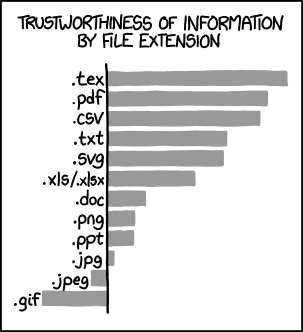
\includegraphics[width=0.4\textwidth,height=\textheight]{images/file_extensions.png}
\caption{\href{https://www.explainxkcd.com/wiki/index.php/1301:_File_Extensions}{XKCD
1301}}
\end{figure}

\end{document}
